\documentclass{beamer}
%
% Choose how your presentation looks.
%
% For more themes, color themes and font themes, see:
% http://deic.uab.es/~iblanes/beamer_gallery/index_by_theme.html
%
\mode<presentation>
{
  \usetheme{Boadilla}      % or try Darmstadt, Madrid, Warsaw, ...
  \usecolortheme{beaver} % or try albatross, beaver, crane, ...
  \usefonttheme{default}  % or try serif, structurebold, ...
  \setbeamertemplate{navigation symbols}{}
  \setbeamertemplate{caption}[numbered]
  
} 

\usepackage{xcolor,colortbl}
\usepackage[english]{babel}
\usepackage[utf8x]{inputenc}
\usepackage{courier}
\usepackage{dsfont}
\usepackage{verbatim} 
\usepackage{enumerate}
\usepackage{tikz}
\usepackage{multirow}
\usepackage{bbm}
\usepackage{venndiagram}
\usepackage{epigraph} 
%\usepackage{xcolor}

%\usepackage{enumitem}

\usepackage{hyperref}
\hypersetup{
    colorlinks=true,
    linkcolor=blue,
    filecolor=magenta,      
    urlcolor=cyan,
}

% R stuff!
\usepackage{listings}
\definecolor{codegreen}{rgb}{0,0.6,0}
\definecolor{codegray}{rgb}{0.5,0.5,0.5}
\definecolor{codepurple}{rgb}{0.58,0,0.82}
\definecolor{backcolour}{rgb}{0.95,0.95,0.92}

\lstdefinestyle{mystyle}{
    backgroundcolor=\color{backcolour},    
    commentstyle=\color{codegreen},
    keywordstyle=\color{black},
    numberstyle=\tiny\color{codegray},
    stringstyle=\color{codepurple},
    basicstyle=\ttfamily\footnotesize,
    breakatwhitespace=false,         
    breaklines=true,                 
    captionpos=b,                    
    keepspaces=true,                 
    numbers=left,                    
    numbersep=5pt,                  
    showspaces=false,                
    showstringspaces=false,
    showtabs=false,                  
    tabsize=2
}

\lstset{style=mystyle}


\setbeamertemplate{enumerate items}[default]
\setbeamertemplate{itemize item}[triangle]

%\setitemize{label=\usebeamerfont*{itemize item}%
%  \usebeamercolor[fg]{itemize item}
%  \usebeamertemplate{itemize item}}



\title[SST-115 / STA-209]{Introduction to Probability}
\subtitle{}
\author{Grinnell College}
\date{October 7, 2024}

\graphicspath{{img/}}

\begin{document}

\begin{frame}
  \titlepage
\end{frame}

\begin{frame}{Review}
A couple of weeks ago we spent some time making tables and using them to answer questions.
\begin{itemize}
    \item What percent of Titanic passengers survived?
    \item What percent of Florida voters supported citizenship pathways for immigrants who entered the US illegally. 
    \item What percent of 30-50 year olds had low job satisfaction?
\end{itemize}
\end{frame}

\begin{frame}{Today's Outline}
\begin{itemize}
    \item continue to use tables of data.
    \item introduce probabilities
    \item probability math
\end{itemize}
\end{frame}

\begin{frame}{What is Probability?}
\textbf{Probabilities} are numbers between 0 and 1 that represent how likely (or unlikely) an \underline{event} is to happen. \vspace{3mm}
\begin{itemize}
    \item closer to zero = more unlikely
    \item closer to one = more likely
\end{itemize} \vspace{5mm}
When multiple events are equally likely, probability can be thought of as a fraction
\begin{align*}
\frac{\text{ \# of ways an event can happen}}{\text{\# of all possible outcomes}}
\end{align*}
\textbf{Examples:}

Flipping a coin: 1 heads out of 2 possibilities $\rightarrow$ prob. heads = 1/2 = 0.5
Probability of rolling an odd number on a 20-sided die?
\end{frame}

\begin{frame}{Types of Probability}
\textbf{Subjective Probability:}
\begin{itemize}
    \item How likely an event is to happen based on someone's personal belief / experience / feelings
    \item Most likely different answers from different people
    \item Ex: prob. of a sports team winning their next game?
\end{itemize}
\end{frame}

\begin{frame}{Types of Probability}
\textbf{Theoretical Probability:}
\begin{itemize}
    \item How likely an event is to happen based on formulas or assumptions about the event
    \item Common assumption: events are equally likely to happen
        \begin{itemize}
            \item coin flips
            \item dice rolling
        \end{itemize}
\end{itemize} \vspace{4mm}
Example:
Suppose there are 20 marbles in a bag. 2 marbles are red, 6 are blue, and 12 are green.
\begin{itemize}
    \item prob. of pulling red marble?
    \item prob. of blue?
    \item prob. of green?
\end{itemize}
\end{frame}

\begin{frame}{Types of Probability}
\textbf{Empirical Probability:}
\begin{itemize}
    \item How likely an event is to happen based on collected data
    \item Sometimes we estimate the probability with data in the form of a table
    \item Ex: flip a coin 1000 times and find the 'empirical' probability of getting a Heads
\end{itemize} \vspace{8mm}

\textbf{Law of Large Numbers:}

If you repeat trials a whole bunch (and they don't affect each other) then the empirical probability will converge to the "true" probability
\end{frame}

\begin{frame}{Empirical Examples}

{\scriptsize A report published in 1988 summarizes results of a Harvard Medical School clinical trial determining effectiveness of asprin in preventing heart attacks in middle-aged male physicians}

\begin{table}
    \centering
    \begin{tabular}{|c|c|c|c|} \hline  
         &  \multicolumn{2}{|c|}{Heart Attack}& \\ \hline  
         Treatment&  Attack&  No Attack& Total\\ \hline  
         Placebo&  189&  10,845& 11,034\\ \hline  
         Aspirin&  104&  10,933& 11,037\\ \hline  
         Total&  293&  21,778& 22,071\\ \hline 
    \end{tabular}
\end{table} \vspace{3mm}
\scriptsize
Probability a randomly selected participant has a heart attack? \vspace{3mm}

(Conditional) Probability a randomly selected participant in the placebo group has a heart attack? \vspace{3mm}

(Conditional) Of those who had a heart attack, what would be the probability of a randomly selected participant being in the placebo group?
\end{frame}

\begin{frame}{Notation}
To save our selves some time, we often use some shorthand notation\vspace{6mm}

P() is used to denote the probability of something, capital letters are quick ways to write down events
\begin{itemize}
    \item P(patient having a heart attack) $\rightarrow$ P(heart attack) $\rightarrow$ P(H)
    \item read as "probability of patient having a heart attack"
\end{itemize} \vspace{8mm}

Often times we may think of an event in terms of "success" (it happened) or "not success" (it did not happen) \vspace{3mm}

Did patient have a heart attack?
\begin{itemize}
    \item Yes = Success (unfortunate terminology)
    \item No = Failure
\end{itemize}
\end{frame}

\begin{frame}{Probability Definitions}
\textbf{Marginal Probability} -- the probability of a single event
\begin{itemize}
    \item P(H) = P(Heart attack)
    \item name comes from using the margins (totals) of a table
\end{itemize}\vspace{8mm}

\textbf{Union} -- 
Scenario where one event happens \textbf{or} another event happens (or both)
\begin{itemize}
    \item We will always use 'inclusive or' meaning both events happening is allowed
    \item denoted P(A or B), P(A $\cup$ B)
\end{itemize} \vspace{8mm}

\textbf{Intersection} -- Scenario where two events happen at the same time
\begin{itemize}
    \item denoted P(A and B), P(A $\cap$ B)
\end{itemize}
\end{frame}

\begin{frame}{Probability Definitions}
\textbf{Conditional Probability} -- probability of event A occuring if event B has already happened
\begin{itemize}
    \item P(A if B), P(A given B), P(A$|$B)
    \item ex: P(Heart attack if patient was given a placebo) = P(HA if placebo)
    \item we look at the 'given' variable first before calculating our probability
\end{itemize}

\begin{table}
    \centering
    \begin{tabular}{|c|c|c|c|} \hline  
         &  \multicolumn{2}{|c|}{Heart Attack}& \\ \hline  
         Treatment&  Attack&  No Attack& Total\\ \hline  
         Placebo&  189&  10,845& 11,034\\ \hline  
         Aspirin&  104&  10,933& 11,037\\ \hline  
         Total&  293&  21,778& 22,071\\ \hline 
    \end{tabular}
\end{table} \vspace{5mm}

\textbf{Independence} -- When one event happening does not affect another
\begin{itemize}
    \item P(A if B) = P(A)
    \item are Attack and Placebo independent?
\end{itemize}
\end{frame}

\begin{frame}{Probability Definitions}
\textbf{Complements} -- when the event doesn't happen
\begin{itemize}
    \item P(A does not happen) = P(not A) = P(A$^C$)
    \item ex: P(no heart attack)
\end{itemize} \vspace{8mm}

\textbf{Disjoint Events} -- Events that cannot both happen
\begin{itemize}
    \item ex: events "Attack" and "No Attack" are disjoint
    \item ex: events "Placebo" and "Aspirin" are disjoint
    \item ex: events "Placebo" and "Attack" are not disjoint
        \begin{itemize}
            \item there were 189 instances of this happening
        \end{itemize}
\end{itemize}
\end{frame}

\begin{frame}{Venn Diagrams}
Venn diagrams can be used as a way to help us think about these probabilities.
\begin{center}
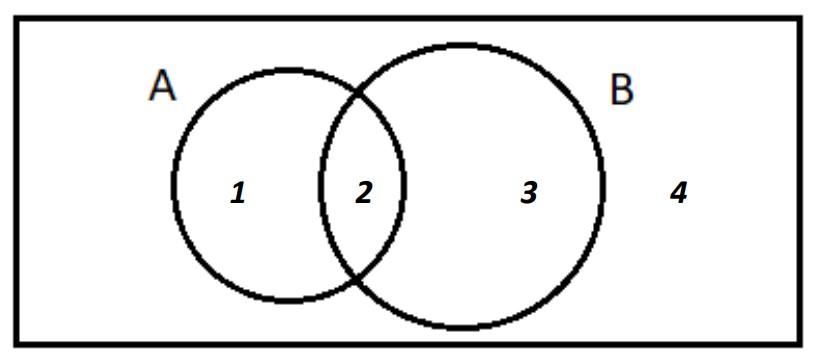
\includegraphics[scale=.5]{img/venn_diagram1.jpg}
\end{center}
\scriptsize{
\begin{enumerate}
    \item Which portion(s) of the Venn Diagram show above is the intersection of A and B? \vspace{4mm}
    \item Which portion(s) of the Venn Diagram show above are the union of A and B? \vspace{4mm}
    \item Which portion(s) of the Venn Diagram show above is the complement of A?
\end{enumerate}}
\end{frame}

\begin{frame}{Venn Diagrams}
\begin{center}
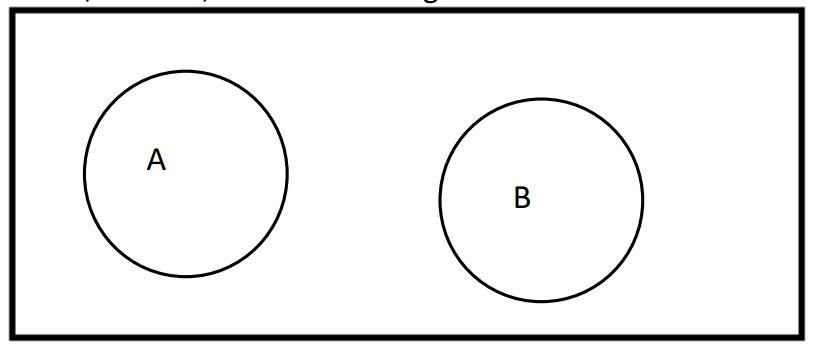
\includegraphics[scale=.5]{img/venn_diagram2.jpg} \vspace{3mm}
\end{center}
\textbf{Disjoint Events} can also be thought of as events that do not overlap
\begin{itemize}
    \item P(A and B) = P(A $\cap$ B) = 0
\end{itemize}
    
\end{frame}


\begin{frame}{Probability Rules / Formulas}
\textbf{Complement Rule}
\begin{itemize}
    \item P(not A) = 1 - P(A)
\end{itemize} \vspace{4mm}

\textbf{Additive Rule}
\begin{itemize}
    \item P(A or B) = P(A) + P(B) - P(A and B)
    \item Special: A and B are disjoint $\rightarrow$ P(A or B) = P(A) + P(B)
\end{itemize} \vspace{4mm}

\textbf{Multiplicative Rule}
\begin{itemize}
    \item P(A and B) = P(A if B)$\times$P(B) = P(B if A)$\times$P(A)
    \item Special: A and B are independent $\rightarrow$ P(A and B) = P(A)$\times$P(B)
\end{itemize} \vspace{4mm}

\textbf{Conditional Probabilities}
\begin{itemize}
    \item probability of A occurring if B has occurred
    \item P(A if B) = $\frac{\textbf{P(A and B)}}{\textbf{P(B)}}$
\end{itemize}
\end{frame}


%\begin{frame}
%\begin{columns}
%
%  \begin{column}{0.45\textwidth}
%%
%  \end{column}
%  \begin{column}{0.45\textwidth}
%%
%  \end{column}
%
%\end{columns}
%\end{frame}


\end{document}
